\documentclass[conference]{IEEEtran}
\IEEEoverridecommandlockouts
\usepackage{cite}
\usepackage{amsmath,amssymb}
\usepackage{graphicx}
\usepackage{booktabs}
\usepackage{url}
\usepackage{xcolor}
\usepackage{balance}
\graphicspath{{figures/}}

\title{Enchanted Ink: An AI Smart Whiteboard}

\author{\IEEEauthorblockN{Arjun C and Anvita Dey}
\IEEEauthorblockA{Electrical and Electronics Department\\
Amrita Vishwa Vidyapeetham\\
Arjun C: AM.EN.U4EEE24016; Anvita Dey: AM.EN.U4EEE24014}}

\begin{document}
\maketitle

\begin{abstract}
Enchanted Ink is an AI-integrated smart whiteboard with Gemini Vision as its external handwriting recognizer. Users write or draw on a Fabric.js canvas; selected ink is sent as an image crop to Gemini for transcription, then an anchored \texttt{@board} command can route the reviewed text to structured board generation. The API validates generated objects before insertion, while ink preservation, object editing, board persistence, and batch undo support a reviewable workflow. Separately, we evaluated the downloaded \texttt{seaandsun/enchanted-ink-trocr} checkpoint offline on 35 held-out line images from a 336-line dataset. This TrOCR experiment measured character error rate (CER) 0.132 (line-bootstrap 95\% interval 0.079--0.212), word error rate (WER) 0.379 (0.280--0.506), and exact-line match 4/35 (11.4\%). These metrics describe the checkpoint experiment, not Gemini recognition or live application accuracy. The line-level split has no writer identifiers and does not establish generalization to unseen writers.
\end{abstract}

\begin{IEEEkeywords}
handwritten text recognition, TrOCR, smart whiteboard, human-in-the-loop, editable canvas
\end{IEEEkeywords}

\section{Introduction}
Digital whiteboards support free-form thinking but leave handwritten ideas difficult to reuse. Conversational AI tools can generate useful material, yet their responses are often separated from the workspace. Enchanted Ink integrates handwriting, AI generation, and native canvas objects in one browser application. The user can write, draw, type an \texttt{@board} instruction, inspect the generated response, and continue editing it on the same canvas.

The live application sends handwriting crops to Gemini Vision for external transcription. A separately configured board-generation provider (Gemini or local Ollama) creates structured objects from explicit commands. Since the Gemini transcription endpoint provides no calibrated confidence score, the interface requires users to review recognized text before command execution. This report separately evaluates the local TrOCR checkpoint offline; it does not report Gemini recognition accuracy, board-generation quality, or end-to-end usability.

\section{System Workflow}
The client is a Fabric.js infinite canvas. It groups nearby pen strokes, rasterizes a crop, and sends it to the FastAPI recognition endpoint. The Gemini Vision service sends this image crop to Google and returns a transcription without a calibrated confidence score. The client preserves the original ink and asks the user to review the text before it can be used as a board command. Image content therefore leaves the local machine during recognition.

An anchored parser recognizes \texttt{@board} at the start of a command. Only then does the board AI service receive the instruction and relevant board context. The response is schema-validated before the client inserts notes, shapes, or connectors as editable Fabric objects. Each generated batch can be undone independently. Boards are stored in SQLite and can be exported as PNG or JSON. Fig.~\ref{fig:workflow} summarizes the pipeline.

\begin{figure*}[t]
\centering
\fbox{\parbox{0.92\textwidth}{\centering
Pen or typed input $\rightarrow$ Gemini Vision transcription $\rightarrow$ user review\\[2pt]
$\rightarrow$ \texttt{@board} command parser $\rightarrow$ structured board generation\\[2pt]
$\rightarrow$ schema validation $\rightarrow$ editable canvas objects, persistence, and undo}}
\caption{Smart-board interaction flow. Handwriting recognition uses external Gemini Vision; TrOCR results elsewhere in this report come from offline checkpoint evaluation.}
\label{fig:workflow}
\end{figure*}

\section{TrOCR Fine-Tuning}
The checkpoint uses a TrOCR vision encoder and autoregressive text decoder, initialized from \texttt{microsoft/trocr-small-stage1}~\cite{li2023trocr}. Saved training arguments specify three epochs, batch size four, gradient accumulation of four steps, AdamW with learning rate $10^{-5}$, linear learning-rate scheduling, weight decay 0.01, FP16, and seed 42. Training and evaluation used the Kaggle English Handwritten Line dataset~\cite{kaggle_english_lines}. The manifest contains 268 training, 33 validation, and 35 test lines. The checkpoint was obtained from \texttt{seaandsun/enchanted-ink-trocr}~\cite{trocr_checkpoint}.

Writer identifiers are unavailable. The split is therefore line-level, not writer-disjoint, and examples from one handwriting style may appear in multiple subsets. Hardware used for fine-tuning was not recorded in the saved checkpoint arguments.

\section{Evaluation Method}
We ran the fine-tuned checkpoint on every line assigned to the fixed test split. All 35 images produced a non-empty transcription. Character error rate and word error rate are Levenshtein edit counts divided by the corresponding number of reference characters and words:
\begin{equation}
\mathrm{CER}=\frac{S_c+D_c+I_c}{N_c},\qquad
\mathrm{WER}=\frac{S_w+D_w+I_w}{N_w},
\end{equation}
where $S$, $D$, and $I$ denote substitutions, deletions, and insertions. Exact-line match is the fraction of test lines whose normalized transcript exactly matches its reference. Character precision, recall, and F1 are computed from aligned character pairs; they are not character-level calibrated probabilities.

We report percentile intervals from 1,000 bootstrap resamples of test lines. These intervals describe resampling variability within this small test set; they do not correct for writer overlap or dataset selection. Inference latency was recorded per line on a 13th Gen Intel Core i3-1315U CPU with 8 GB system memory. Confidence calibration and board-command execution metrics were not evaluated.

\section{Results}
Table~\ref{tab:metrics} reports aggregate held-out metrics. The checkpoint returned a transcript for each test image. It exactly matched four full reference lines, even though aggregate character alignment was substantially higher; word-level errors remain more frequent than character-level errors.

\begin{table}[t]
\caption{TrOCR Results on the 35-Line Test Split}
\label{tab:metrics}
\centering
\small
\begin{tabular}{lr}
\toprule
Measure & Result \\
\midrule
Character error rate & 0.132 (95\% CI: 0.079--0.212) \\
Word error rate & 0.379 (95\% CI: 0.280--0.506) \\
Exact-line match & 4/35 (11.4\%) \\
Character alignment accuracy & 0.868 \\
Character micro-F1 & 0.917 \\
Character macro-F1 & 0.666 \\
Word micro-F1 & 0.730 \\
Mean / median / P95 latency & 12.35 / 11.46 / 20.02 s \\
\bottomrule
\end{tabular}
\end{table}

Fig.~\ref{fig:confusion} shows aligned counts for the most common reference characters. It uses a logarithmic color scale and preserves off-diagonal substitutions; it is not row-normalized. Fig.~\ref{fig:errors} shows character substitutions, insertions, and deletions. The observed 125 character insertions are the largest of these edit categories for this run.

\begin{figure*}[t]
\centering
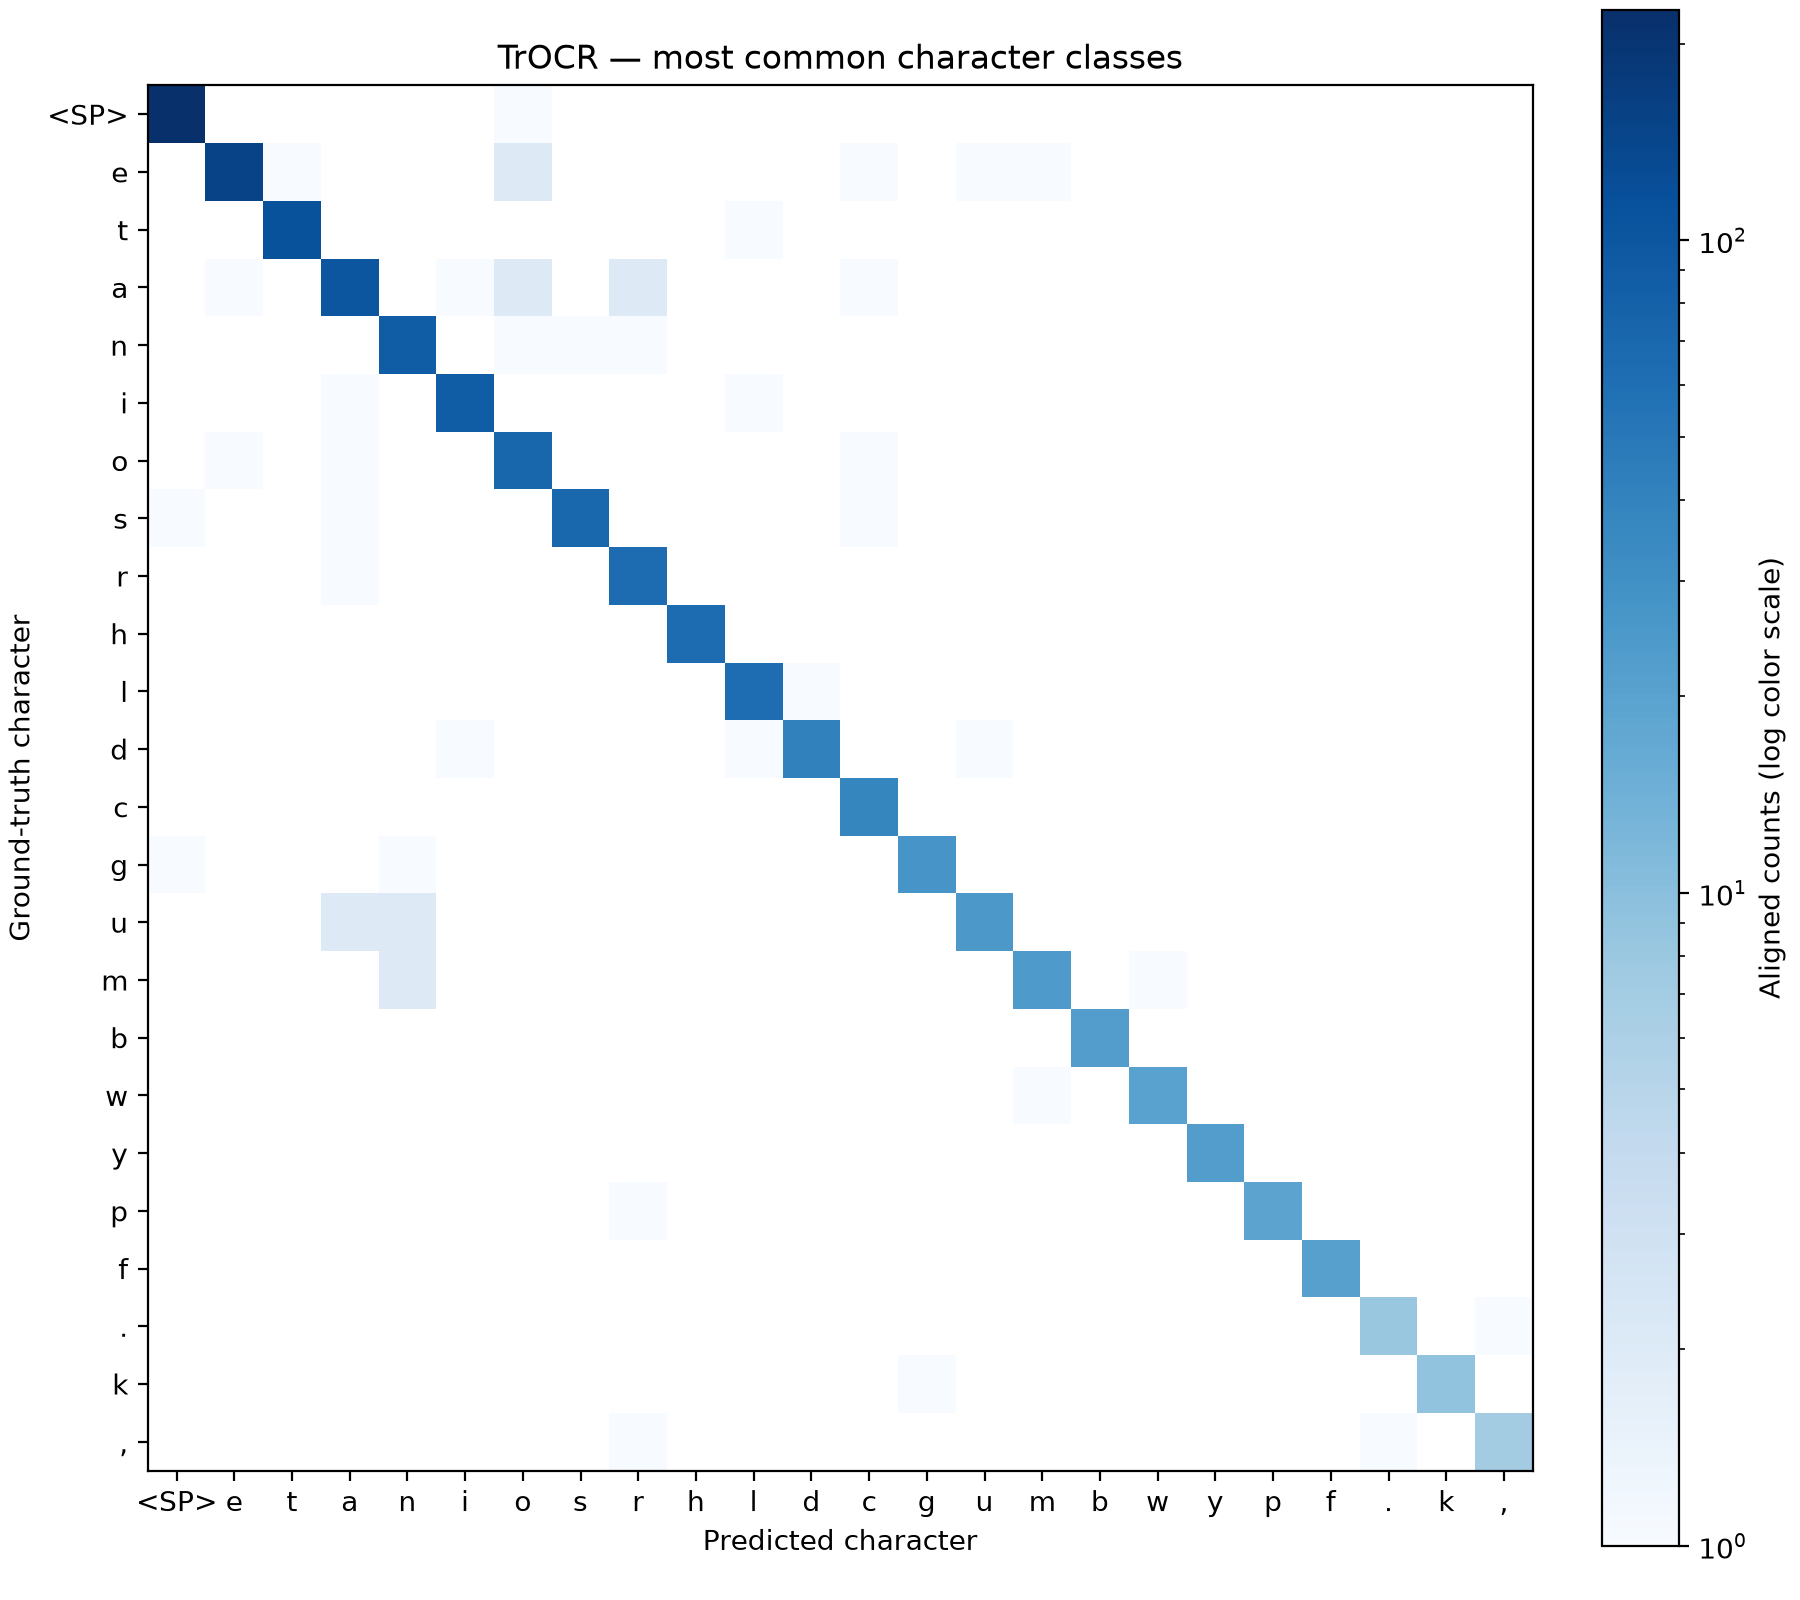
\includegraphics[width=0.72\textwidth]{confusion_trocr.png}
\caption{TrOCR aligned character confusion counts for frequent character classes. Color represents raw counts on a logarithmic scale.}
\label{fig:confusion}
\end{figure*}

\begin{figure}[t]
\centering
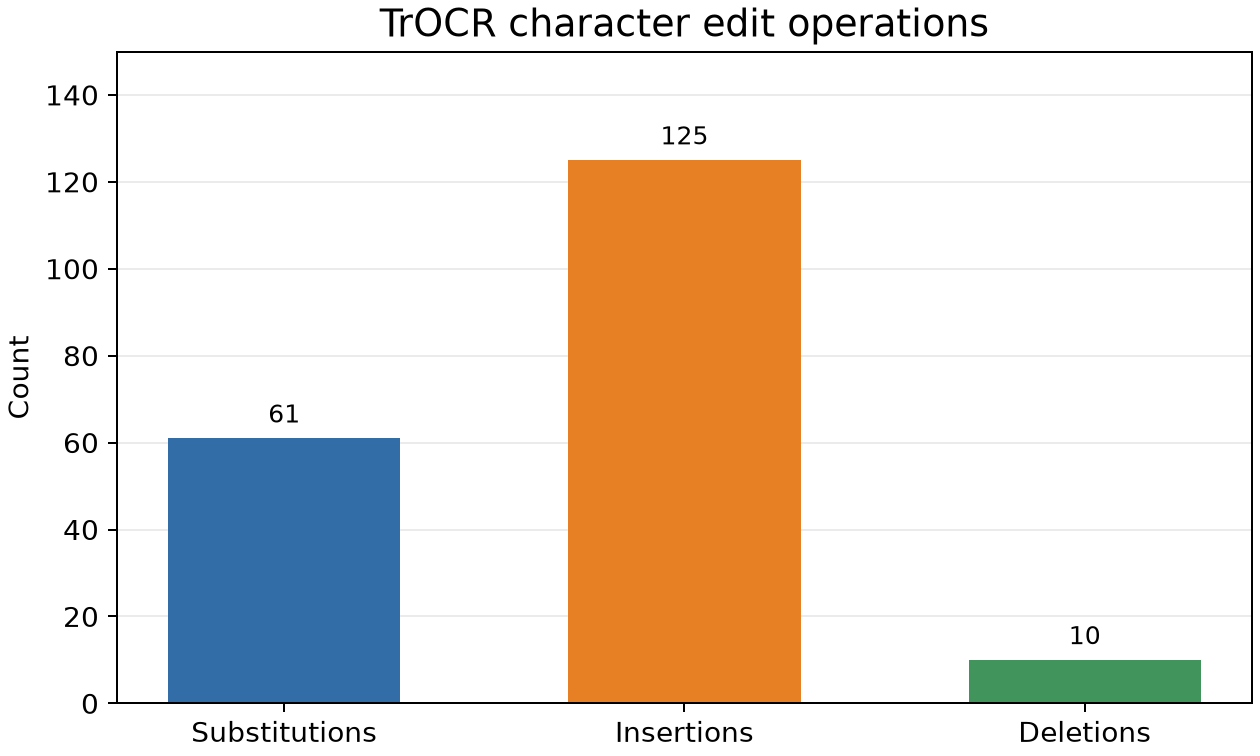
\includegraphics[width=\columnwidth]{error_breakdown.png}
\caption{Character edit operations over all 35 test lines.}
\label{fig:errors}
\end{figure}

\begin{figure}[t]
\centering
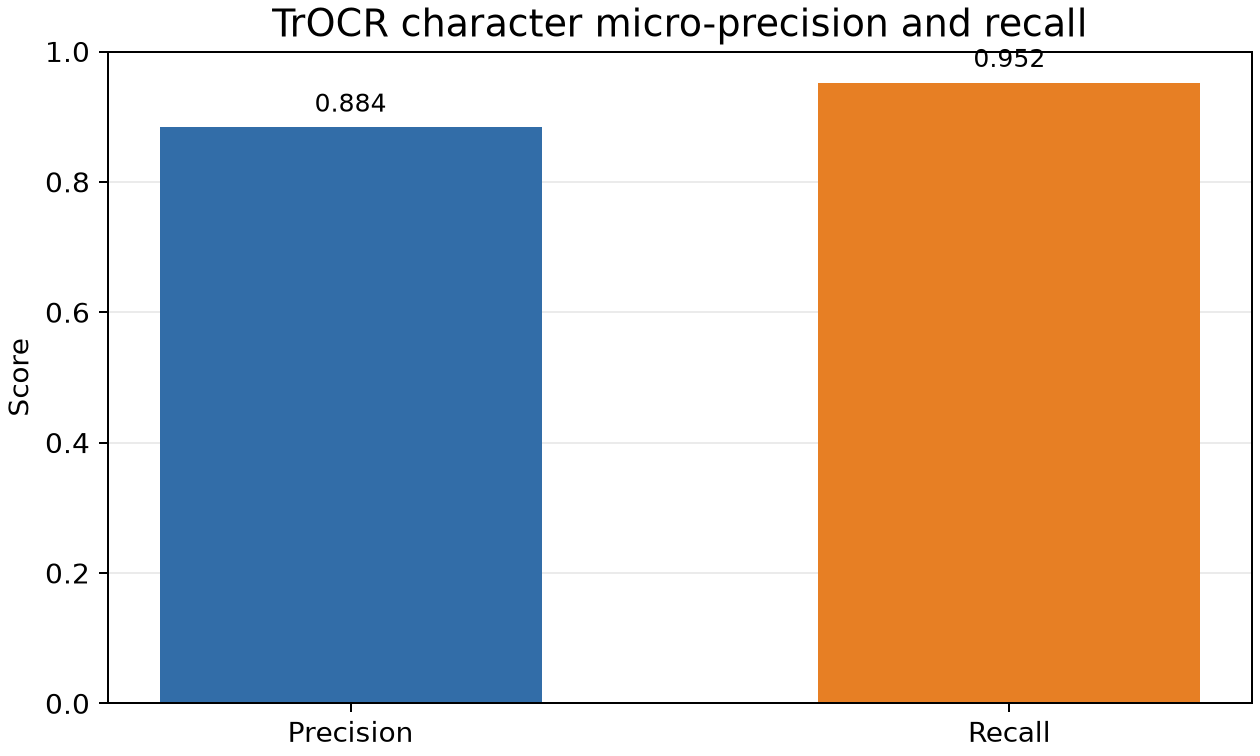
\includegraphics[width=\columnwidth]{precision_recall.png}
\caption{Character micro-precision and micro-recall from sequence alignment.}
\label{fig:pr}
\end{figure}

\begin{figure}[t]
\centering
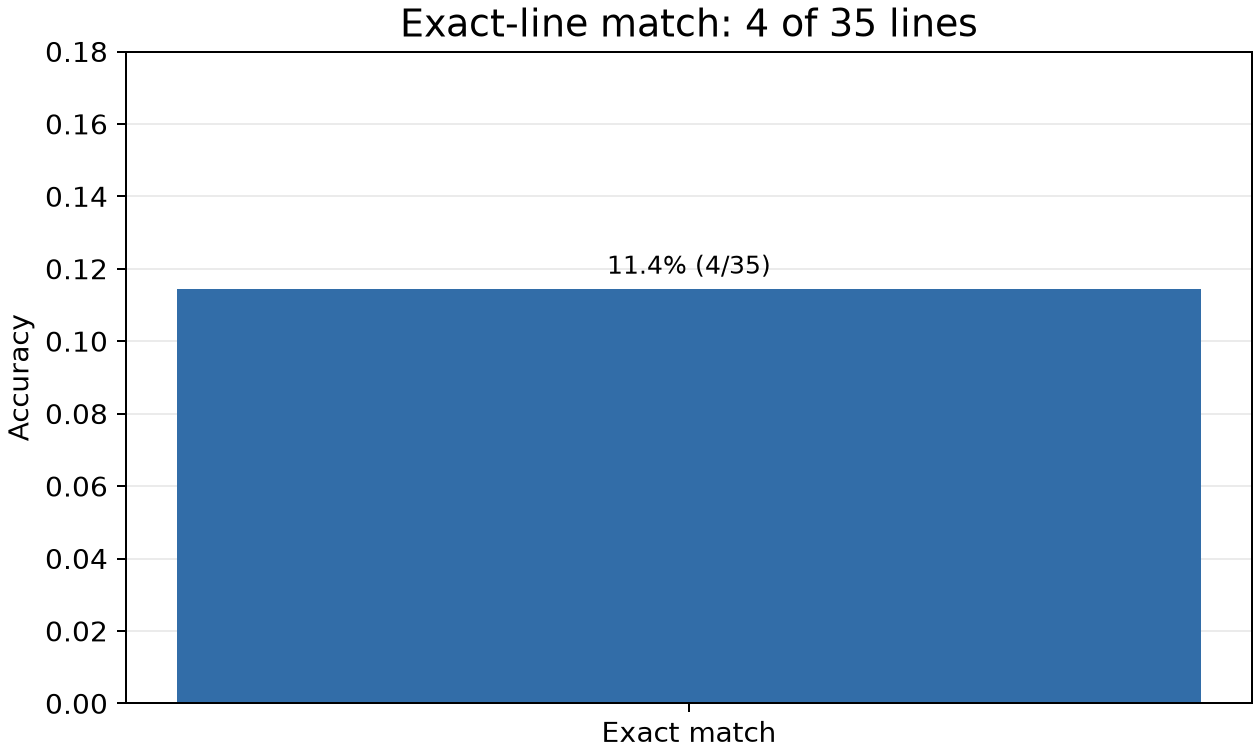
\includegraphics[width=\columnwidth]{exact_line_accuracy.png}
\caption{Exact-line accuracy; four of 35 lines matched exactly.}
\label{fig:exact}
\end{figure}

\section{Discussion and Limitations}
The offline TrOCR benchmark is a model experiment and is not the live recognizer in the current application. Its 11.4\% exact-line match shows that complete line transcription often differs from the reference, while WER 0.379 indicates substantial word-level error. The live Gemini recognizer has not been benchmarked here and returns no calibrated confidence, so confirmation and ink preservation remain important safeguards.

This experiment has several limits. The sample contains only 35 test lines; the bootstrap intervals are consequently broad. Missing writer IDs prevent a writer-independent estimate. The dataset license was not recorded in the local manifest. The evaluation is line-level and does not assess page layout analysis, board-command detection accuracy, object-generation quality, task success, or user correction effort. The recorded model latency is specific to the local CPU and the current inference settings. No comparison against another recognizer is claimed.

A stronger follow-up should use a larger licensed dataset with writer-disjoint train, validation, and test partitions, preserve the exact training environment and revision, and measure command transcription and correction effort in the application.

\section{Conclusion}
Enchanted Ink integrates Gemini Vision handwriting transcription with structured AI generation inside an editable and reversible whiteboard. An offline TrOCR evaluation on 35 held-out lines measured CER 0.132, WER 0.379, and exact-line match 4/35; these scores do not measure Gemini or live application performance. A larger writer-disjoint test and an end-to-end evaluation of the deployed recognizer are needed next.

\section*{Reproducibility}
The project repository is available at \url{https://github.com/arjuncdev/Enchanted_Ink}. Aggregate test metrics, PNG figures, saved checkpoint arguments, and the evaluation command are included with the submission artifacts. Source images and the test manifest are not included because sharing rights have not been verified. The checkpoint is linked in the bibliography. \balance

\bibliographystyle{IEEEtran}
\bibliography{references}
\end{document}
